\begin{lemma}{Three Tangents Lemma}{}
	Let $ABC$ be an acute triangle. Let $BE$ and $CF$ be altitudes of
	$\triangle{ABC}$, and denote by $M$ the midpoint of $BC$. Prove that $ME$, $MF$,
	and the line through $A$ parallel to $BC$ are all tangents to $(AEF)$.
\end{lemma}
\begin{centering}
	% Aceita "linewidth=0.6pt/g" (export típico do GeoGebra) e converte para "line width=0.6pt"
\tikzset{linewidth/.style args={#1/g}{line width=#1}}
\definecolor{qqwuqq}{rgb}{0,0.39215686274509803,0}
\definecolor{xdxdff}{rgb}{0.49019607843137253,0.49019607843137253,1}
\definecolor{ffqqqq}{rgb}{1,0,0}
\definecolor{qqzzqq}{rgb}{0,0.6,0}
\definecolor{qqqqff}{rgb}{0,0,1}
\begin{tikzpicture}[scale=0.7,line cap=round,line join=round,>=triangle 45,x=1cm,y=1cm]
	\clip(-13.479734933638587,-0.27847742737593095) rectangle (6.128228152397923,10.49436817401107);
	\draw [shift={(-6,10)},linewidth=0.6pt/g,color=ffqqqq,fill=ffqqqq,fill opacity=0.1] (0,0) -- (-48.01278750418334:0.3460228779888796) arc (-48.01278750418334:0:0.3460228779888796) -- cycle;
	\draw [shift={(-6,3.6)},linewidth=0.6pt/g,color=ffqqqq,fill=ffqqqq,fill opacity=0.1] (0,0) -- (41.98721249581666:0.3460228779888796) arc (41.98721249581666:90:0.3460228779888796) -- cycle;
	\draw [shift={(-8.206896551724139,4.482758620689655)},linewidth=0.6pt/g,color=ffqqqq,fill=ffqqqq,fill opacity=0.1] (0,0) -- (20.18580300946485:0.3460228779888796) arc (20.18580300946485:68.19859051364818:0.3460228779888796) -- cycle;
	\draw [shift={(3,0)},linewidth=0.6pt/g,color=ffqqqq,fill=ffqqqq,fill opacity=0.1] (0,0) -- (131.98721249581666:0.3460228779888796) arc (131.98721249581666:180:0.3460228779888796) -- cycle;
	\draw [shift={(-2.81767955801105,6.464088397790055)},linewidth=0.6pt/g,color=qqwuqq,fill=qqwuqq,fill opacity=0.10000000149011612] (0,0) -- (-159.81419699053518:0.3460228779888796) arc (-159.81419699053518:-138.01278750418336:0.3460228779888796) -- cycle;
	\draw [shift={(-6,10)},linewidth=0.6pt/g,color=qqwuqq,fill=qqwuqq,fill opacity=0.10000000149011612] (0,0) -- (-111.80140948635183:0.3460228779888796) arc (-111.80140948635183:-90:0.3460228779888796) -- cycle;
	\draw [shift={(-2.81767955801105,6.464088397790055)},linewidth=0.6pt/g,color=qqqqff,fill=qqqqff,fill opacity=0.1] (0,0) -- (-138.01278750418336:0.3460228779888796) arc (-138.01278750418336:-96.02557500836669:0.3460228779888796) -- cycle;
	\draw [shift={(-10,0)},linewidth=0.6pt/g,color=qqqqff,fill=qqqqff,fill opacity=0.1] (0,0) -- (0:0.3460228779888796) arc (0:41.98721249581666:0.3460228779888796) -- cycle;
	\draw [shift={(-8.206896551724139,4.482758620689655)},linewidth=0.6pt/g,color=qqqqff,fill=qqqqff,fill opacity=0.1] (0,0) -- (-21.801409486351808:0.3460228779888796) arc (-21.801409486351808:20.185803009464852:0.3460228779888796) -- cycle;
	\draw [shift={(-6,10)},linewidth=0.6pt/g,color=qqqqff,fill=qqqqff,fill opacity=0.1] (0,0) -- (-90:0.3460228779888796) arc (-90:-48.012787504183336:0.3460228779888796) -- cycle;
	\draw [linewidth=0.6pt/g,color=qqqqff] (-6,10)-- (-10,0);
	\draw [linewidth=0.6pt/g,color=qqqqff] (-10,0)-- (3,0);
	\draw [linewidth=0.6pt/g,color=qqqqff] (3,0)-- (-6,10);
	\draw [linewidth=0.6pt/g,color=qqzzqq] (3,0)-- (-8.206896551724139,4.482758620689655);
	\draw [linewidth=0.6pt/g,color=qqzzqq] (-10,0)-- (-2.81767955801105,6.464088397790055);
	\draw [linewidth=0.6pt/g,color=ffqqqq] (-6,6.8) circle (3.2cm);
	\draw [linewidth=0.6pt/g,color=qqzzqq] (-3.5,0)-- (-8.206896551724139,4.482758620689655);
	\draw [linewidth=0.6pt/g,color=qqzzqq] (-3.5,0)-- (-2.81767955801105,6.464088397790055);
	\draw [linewidth=0.6pt/g,color=qqzzqq] (-3.2306889125105824,3.210632838489085) -- (-3.093044452758099,3.196103701070769);
	\draw [linewidth=0.6pt/g,color=qqzzqq] (-3.2246351052529496,3.2679846967192865) -- (-3.086990645500466,3.25345555930097);
	\draw [shift={(-6,10)},linewidth=0.6pt/g,color=ffqqqq] (-48.01278750418334:0.3460228779888796) arc (-48.01278750418334:0:0.3460228779888796);
	\draw[linewidth=0.6pt/g,color=ffqqqq] (-5.723419569145305,9.876821474219552) -- (-5.644396588901106,9.841627609710853);
	\draw [linewidth=0.6pt/g,color=ffqqqq] (-6,10)-- (-6,3.6);
	\draw [linewidth=0.6pt/g,color=ffqqqq] (-8.206896551724139,4.482758620689655)-- (-2.81767955801105,6.464088397790055);
	\draw [shift={(-6,3.6)},linewidth=0.6pt/g,color=ffqqqq] (41.98721249581666:0.3460228779888796) arc (41.98721249581666:90:0.3460228779888796);
	\draw[linewidth=0.6pt/g,color=ffqqqq] (-5.876821474219548,3.8765804308547) -- (-5.841627609710848,3.9556034110988993);
	\draw [shift={(-8.206896551724139,4.482758620689655)},linewidth=0.6pt/g,color=ffqqqq] (20.18580300946485:0.3460228779888796) arc (20.18580300946485:68.19859051364818:0.3460228779888796);
	\draw[linewidth=0.6pt/g,color=ffqqqq] (-7.98980876843795,4.69380974789134) -- (-7.927783687499039,4.754110069948964);
	\draw [shift={(3,0)},linewidth=0.6pt/g,color=ffqqqq] (131.98721249581666:0.3460228779888796) arc (131.98721249581666:180:0.3460228779888796);
	\draw[linewidth=0.6pt/g,color=ffqqqq] (2.723419569145305,0.12317852578044718) -- (2.644396588901106,0.15837239028914674);
	\draw [linewidth=0.6pt/g,color=qqqqff] (-3.5,0)-- (-10,0);
	\draw [linewidth=0.6pt/g,color=qqqqff] (-6.721164760167593,-0.06920457559777517) -- (-6.721164760167593,0.06920457559777517);
	\draw [linewidth=0.6pt/g,color=qqqqff] (-6.778835239832405,-0.06920457559777517) -- (-6.778835239832405,0.06920457559777517);
	\draw [linewidth=0.6pt/g,color=qqqqff] (-3.5,0)-- (3,0);
	\draw [linewidth=0.6pt/g,color=qqqqff] (-0.2788352398324071,0.06920457559777517) -- (-0.2788352398324071,-0.06920457559777517);
	\draw [linewidth=0.6pt/g,color=qqqqff] (-0.22116476016759382,0.06920457559777517) -- (-0.22116476016759382,-0.06920457559777517);
	\draw [shift={(-2.81767955801105,6.464088397790055)},linewidth=0.6pt/g,color=qqqqff] (-138.01278750418336:0.3460228779888796) arc (-138.01278750418336:-96.02557500836669:0.3460228779888796);
	\draw [shift={(-2.81767955801105,6.464088397790055)},linewidth=0.6pt/g,color=qqqqff] (-138.01278750418336:0.27105125442462236) arc (-138.01278750418336:-96.02557500836669:0.27105125442462236);
	\draw [shift={(-10,0)},linewidth=0.6pt/g,color=qqqqff] (0:0.3460228779888796) arc (0:41.98721249581666:0.3460228779888796);
	\draw [shift={(-10,0)},linewidth=0.6pt/g,color=qqqqff] (0:0.27105125442462236) arc (0:41.98721249581666:0.27105125442462236);
	\draw [shift={(-8.206896551724139,4.482758620689655)},linewidth=0.6pt/g,color=qqqqff] (-21.801409486351808:0.3460228779888796) arc (-21.801409486351808:20.185803009464852:0.3460228779888796);
	\draw [shift={(-8.206896551724139,4.482758620689655)},linewidth=0.6pt/g,color=qqqqff] (-21.801409486351808:0.27105125442462236) arc (-21.801409486351808:20.185803009464852:0.27105125442462236);
	\draw [shift={(-6,10)},linewidth=0.6pt/g,color=qqqqff] (-90:0.3460228779888796) arc (-90:-48.012787504183336:0.3460228779888796);
	\draw [shift={(-6,10)},linewidth=0.6pt/g,color=qqqqff] (-90:0.27105125442462236) arc (-90:-48.012787504183336:0.27105125442462236);
	\draw [linewidth=0.6pt/g] (-10,10)-- (3,10);
	\begin{scriptsize}
		\draw [fill=black] (-10,0) circle (2.5pt);
		\draw[color=black] (-10.250188072409044,0.20018755384201395) node {$B$};
		\draw [fill=black] (3,0) circle (2.5pt);
		\draw[color=black] (3.094760922028745,0.24632393757386406) node {$C$};
		\draw [fill=black] (-6,10) circle (2.5pt);
		\draw[color=black] (-5.913368001615087,10.246385111452375) node {$A$};
		\draw [fill=black] (-2.81767955801105,6.464088397790055) circle (2pt);
		\draw[color=black] (-2.6030824688548058,6.61314489256918) node {$E$};
		\draw [fill=black] (-8.206896551724139,4.482758620689655) circle (2pt);
		\draw[color=black] (-8.5,4.2) node {$F$};
		\draw [fill=black] (-3.5,0) circle (2pt);
		\draw[color=black] (-3.2374577451677515,0.2693921294397891) node {$M$};
		\draw [fill=xdxdff] (21.743909671462525,10) circle (2.5pt);
		\draw[color=xdxdff] (-13.433598549906737,10.627010277240139) node {$D$};
		\draw [fill=black] (-6,3.6) circle (2pt);
		\draw[color=black] (-5.9710384812799004,3.395132127272634) node {$O$};
	\end{scriptsize}
\end{tikzpicture}

\end{centering}

\begin{lemma}{Iran Lemma}{}
	The incircle of $\triangle{ABC}$ is tangent to $BC, CA, AB$ at $D, E, F$, respectively. Let $M$ and $N$ be the midpoints of $BC$ and $AC$, respectively. Ray $BI$ meets line $EF$ at $K$. Show that $BK \perp CK$. Then show $K$ lies on line $MN$.
\end{lemma}
\begin{figure}[h]
	\centering
	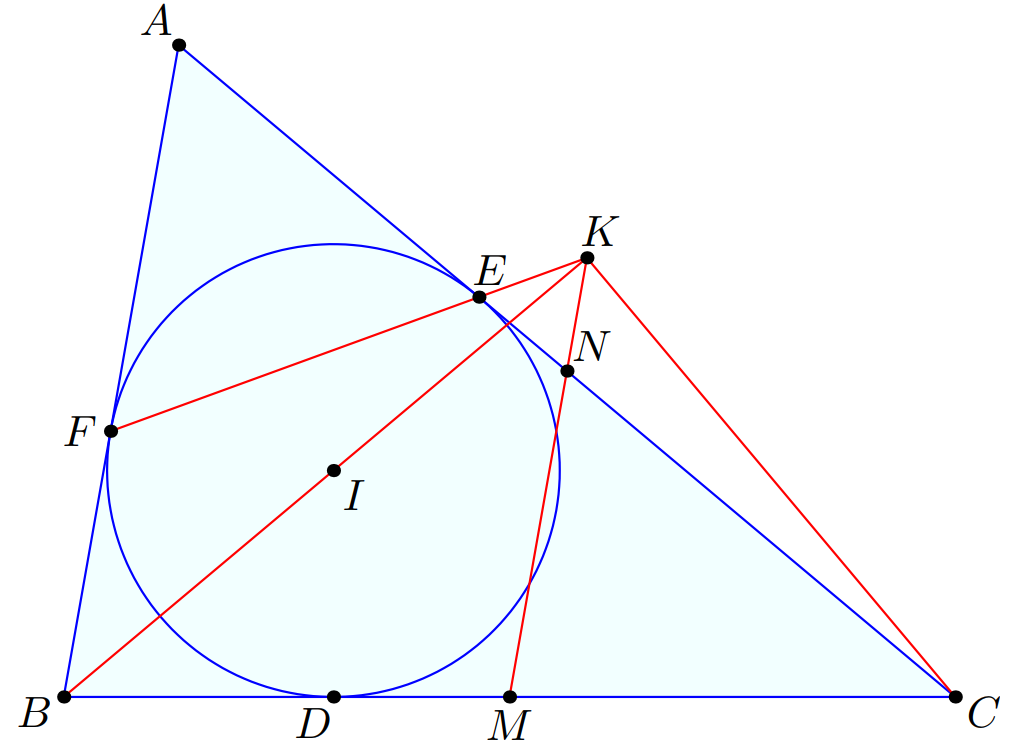
\includegraphics[width=0.5\textwidth]{./img/lemmas/iranlemma}
\end{figure}

\textbf{\textcolor{color2}{Solution.}}
\begin{claim}
	$BK \perp CK$
\end{claim}

\begin{proof}
	Since $F$ and $D$ are reflected over $BI$, the following is true.
	\[
		\measuredangle KDC = \measuredangle BDK = \measuredangle KFB = \measuredangle EFA = \measuredangle AEF = \measuredangle CEK. \qedhere
	\]
\end{proof}

\begin{claim}
	$K$ lies on line $MN$.
\end{claim}

\begin{proof}
	Since $M$ is the circumcenter of $(BKC)$, $\measuredangle CMK = 2 \measuredangle CBK = \measuredangle CBA$. Hence,
	$KM \parallel AB$. However, $MN \parallel AB$. Thus, $N \in KM$.
\end{proof}

\clearpage

\subsubsection{USAJMO 2011 P5}
\begin{problem}
Points $A,B,C,D,E$ lie on a circle $\omega$ and point $P$ lies outside the circle. The given points are such that
\begin{enumerate}[label={(\roman*)}]
	\item lines $PB$ and $PD$ are tangent to $\omega$,
	\item$P, A, C$ are collinear, and
	\item$DE \parallel AC$.
\end{enumerate}
Prove that $BE$ bisects $AC$.
\end{problem}

\begin{figure}[h]
	\centering
	\input{./img/sols/11JMO5}
\end{figure}

\clearpage

\subsubsection{Shortlist 2010 G1}

\begin{problem}
Let $ABC$ be an acute triangle with $D, E, F$ the feet of the altitudes
lying on $BC, CA, AB$ respectively. One of the intersection points of the
line $EF$ and the circumcircle is $P.$ The lines $BP$ and $DF$ meet at point
$Q.$ Prove that $AP = AQ$.
\end{problem}

\begin{figure}[h]
	\centering
	\input{./img/sols/10SLG1}
\end{figure}

Let $\measuredangle$ denote directed angles mod $180^{\circ}$. The line EF meets
the circumcircle at two points. Directed angles allow us to treat both
at once, so we fix one of them.

Our goal is to show $\measuredangle PQA = \measuredangle APQ$, i.e., that $\triangle
	APQ$ is isosceles. We will first prove that $A$, $F$, $P$, $Q$ are concyclic.

Since $\triangle DEF$ is an orthic triangle, $\measuredangle CFA = \measuredangle
	ADC = 90^{\circ}$. Therefore, $FACD$ is cyclic, culminating in $\measuredangle
	ACD = \measuredangle AFD = \measuredangle AFQ$. However, $APCB$ is
cyclic, so $\measuredangle APB = \measuredangle ACB =
	\measuredangle ACD$. Thus, $\measuredangle APQ = \measuredangle AFQ$. Which
means that $AFPQ$ is a cyclic quadrilateral.

$FECB$ is a cyclic quadrilateral either, by the same $FACD$'s reason.
Therefore, putting together everything we've seen so far:

\[
	\measuredangle PQA = \measuredangle PFA = \measuredangle EFB = \measuredangle ECB
	= \measuredangle ACB = \measuredangle APB.
\]
Hence, $AP=AQ$.

\clearpage
\subsubsection{Euler's Lemma}
\begin{figure}[h]
	\centering
	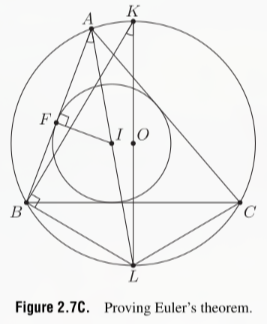
\includegraphics[width=0.6\textwidth]{./img/sols/euler2}
\end{figure}
\begin{figure}[h]
	\centering
	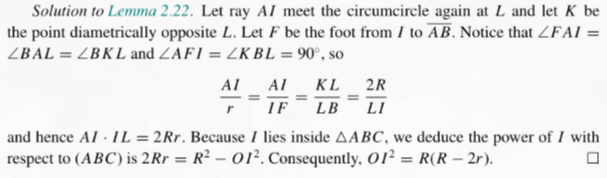
\includegraphics[width=0.6\textwidth]{./img/sols/euler}
\end{figure}

\subsubsection{All-Russian MO 2011}
\begin{figure}[h]
	\centering
	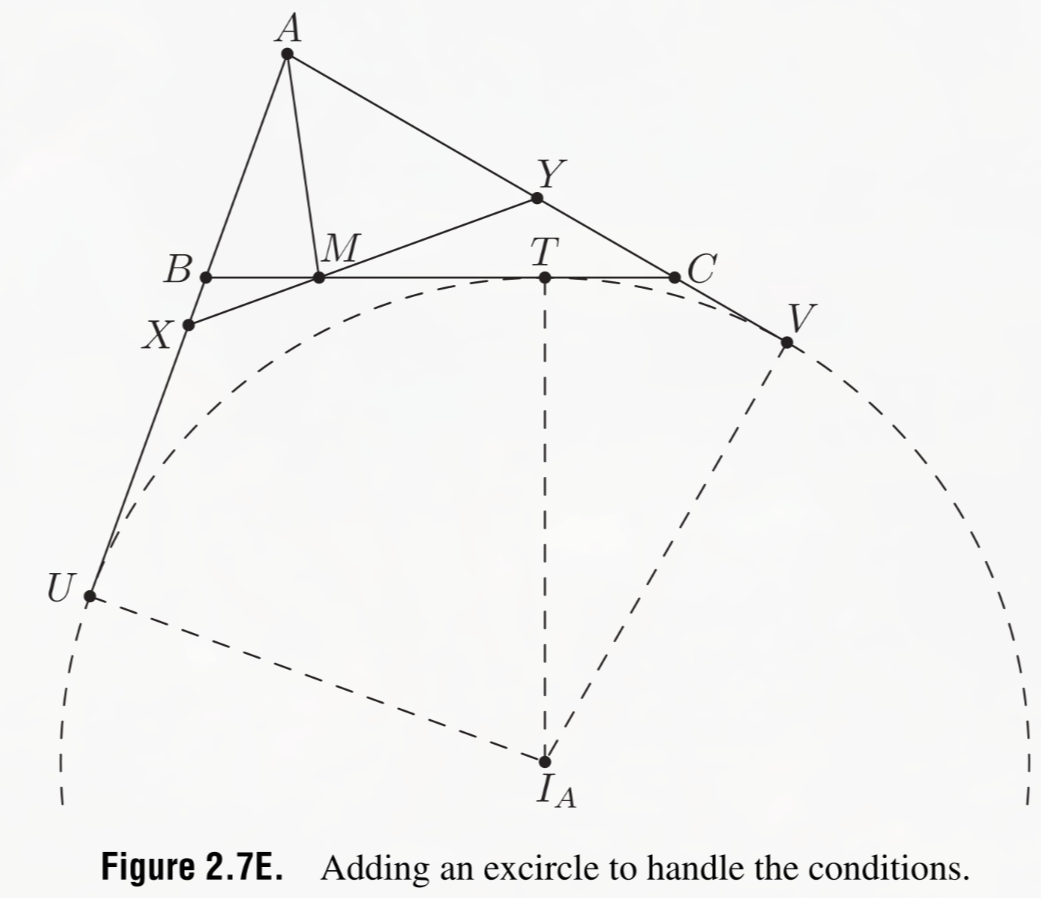
\includegraphics[width=0.6\textwidth]{./img/sols/rus1}
\end{figure}
\begin{figure}[h]
	\centering
	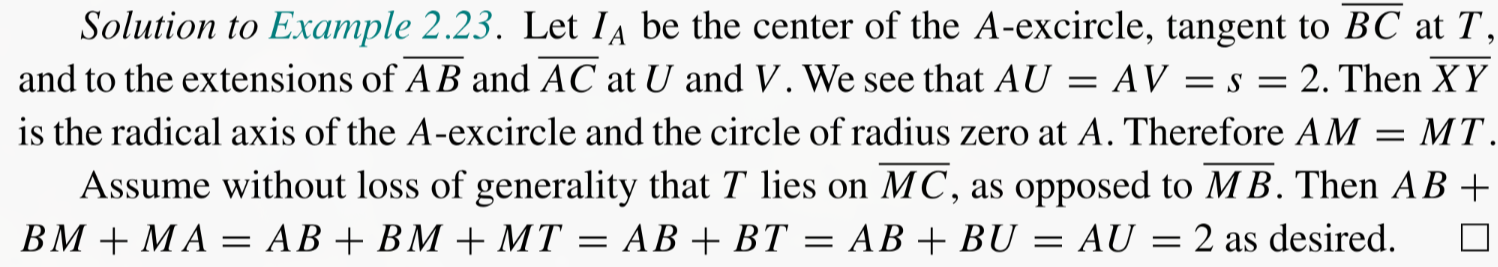
\includegraphics[width=0.6\textwidth]{./img/sols/rus}
\end{figure}

\clearpage

\subsubsection{Iran TST 2011/1 02/13/2026}
\begin{problem}
In acute triangle $ABC$, $\angle B>\angle C$.
Let $M$ be the midpoint of $\overline{BC}$ and let $E$ and $F$ be the feet of the altitudes from $B$ and $C$, respectively.
Let $K$ and $L$ be the midpoints of $\overline{ME}$ and $\overline{MF}$, respectively, and let $T$ lie on line $KL$ such that $\overline{TA}\parallel \overline{BC}$.
Prove that $TA=TM$.
\end{problem}
\begin{figure}[h]
	\centering
	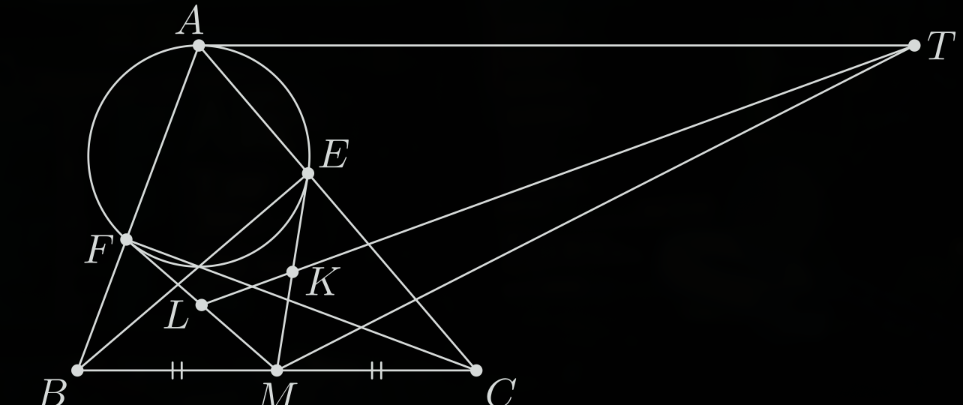
\includegraphics[width=0.6\textwidth]{./img/sols/iran}
\end{figure}
Let $\Gamma_1=(AFE)$ and $\Gamma_2$ be the circumference of radius $0$  centered at $M$. In order to prove $TA=TM$, it is enough to demonstrate that $\operatorname{Pow}_{\Gamma_1}(T)=\operatorname{Pow}_{\Gamma_2}(T)$.
\begin{claim}
	$\overline{KL}$ is the radical axis of $\Gamma_1$ and $\Gamma_2$.
\end{claim}
\begin{proof}
	By the Three Tangents Lemma, $\overline{ME}$ and $\overline{MF}$ are both tangents to $\Gamma_1$. Since, $MK=KE$,
	\[
		\operatorname{Pow}_{\Gamma_1}(K)=\operatorname{Pow}_{\Gamma_2}(K).
	\]
	Hence,
	$K$ lies inside the radical axis of $\Gamma_1$ and $\Gamma_2$. However, we can use an analogous argument to prove that $L$ does either. Hence $\overline{KL}$ is the radical axis of $\Gamma_1$ and $\Gamma_2$.
\end{proof}
Since $K$, $L$ and $M$ are collinear, $M$ lies inside this radical axis too. Hence, $TA=TM$

\clearpage

\subsubsection{02/13/26}
\begin{problem}
Let $\overline{AD}$, $\overline{BE}$, $\overline{CF}$ be the altitudes of a scalene triangle $ABC$ with circumcenter $O$. Prove that $(AOD)$, $(BOE)$, and $(COF)$ intersect at point $X$ other than $O$.
\end{problem}
\begin{figure}[h]
	\centering
	
\includegraphics[width=0.6\textwidth]{img/sols/1.png}
\end{figure}
Let $H$ be the orthocenter $\triangle ABC$. Hence,
\[
	HA \cdot HD = HB \cdot BE = HC \cdot HF,
\]
is true by considering the circumcenters of diameters $AB$, $BC$ and $CA$.
Which means that both $O$ and $H$ have the same power of point of all the circumferences $(AOD)$, $(BOE)$, and $(COF)$.

Hence, those three circumferences have the same radical axis, resulting in another point $X$ where they three intersect.

\clearpage

\subsubsection{BAMO 2012/4 03/04/26}
\begin{problem}
Given a segment $\overline{AB}$ in the plane, choose on it a point $M$ different from $A$ and $B$. Two equilateral triangles $AMC$ and $BMD$ in the plane are constructed on the same side of segment $\overline{AB}$. The circumcircles of the two triangles intersect in point $M$ and another point $N$.

\begin{enumerate}
	\item[(a)] Prove that $AD$ and $BC$ pass through point $N$.
	\item[(b)] Prove that no matter where one chooses the point $M$ along segment $\overline{AB}$, all lines $MN$ will pass through some fixed point $K$ in the plane.
\end{enumerate}
\end{problem}
\begin{figure}[h]
	\centering
	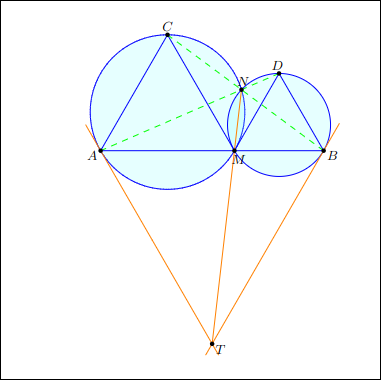
\includegraphics[width=0.5\textwidth]{./img/sols/bamo}
\end{figure}
\begin{enumerate}
	\item[(a)] It is enough to prove that $\measuredangle MNC = \measuredangle MNB$, which is obviously true, since
	      $\measuredangle MNC = \measuredangle CAM = 60^{\circ}$ and $\measuredangle MNB = \measuredangle MDB = 60^{\circ}$.

	\item[(b)] Let $T$ be a point in the opposite side of $D$ and $C$, where $\triangle ATB$ is equilateral.
	      Hence, $TA$ is tangent to $(AMC)$ because $\measuredangle TAB=\measuredangle ACM$.
	      Analogous arment shows that $TB$ is tangent to $(BMD)$. Hence, independent of $M,N$, $T$ lies on
	      the radical axis of $(AMC)$ and $(BMD)$.
\end{enumerate}

\clearpage

\subsubsection{1.12.6 03/04/26}
\begin{problem}
Let $a,b$ be positive integers such that there exists a prime $p$ with the property
\[
	\operatorname{lcm}(a,a+p)=\operatorname{lcm}(b,b+p).
\]
Prove that $a=b$. Hints: 59 281 261
\end{problem}
